
% utf-8 ru, unix eolns
\documentclass[12pt,a4paper,oneside]{extarticle}
    \righthyphenmin=2 %минимально переносится 2 символа %%%
    \sloppy

% Рукопись оформлена в соответствии с правилами оформления 
% электронной версии авторского оригинала, 
% принятыми в Издательстве МГТУ им. Н.Э. Баумана.

\usepackage{geometry} % А4, примерно 28-31 строк(а) на странице 
    \geometry{paper=a4paper}
    \geometry{includehead=false} % Нет верх. колонтитула
    \geometry{includefoot=true}  % Есть номер страницы
    \geometry{bindingoffset=0mm} % Переплет    : 0  мм
    \geometry{top=20mm}          % Поле верхнее: 20 мм
    \geometry{bottom=25mm}       % Поле нижнее : 25 мм 
    \geometry{left=25mm}         % Поле левое  : 25 мм
    \geometry{right=25mm}        % Поле правое : 25 мм
    \geometry{headsep=10mm}  % От края до верх. колонтитула: 10 мм
    \geometry{footskip=20mm} % От края до нижн. колонтитула: 20 мм 

\usepackage{cmap}
\usepackage[T2A]{fontenc} 
\usepackage[utf8x]{inputenc}
\usepackage[english,russian]{babel}
\usepackage{misccorr}

\usepackage{amsmath}
\usepackage{amsfonts}
\usepackage{amssymb}

%\usepackage{cm-super} %человеческий рендер русских шрифтов

\setlength{\parindent}{1.25cm}  % Абзацный отступ: 1,25 см
\usepackage{indentfirst}        % 1-й абзац имеет отступ

\usepackage{setspace}   

\onehalfspacing % Полуторный интервал между строками

\makeatletter
\renewcommand{\@oddfoot }{\hfil\thepage\hfil} % Номер стр.
\renewcommand{\@evenfoot}{\hfil\thepage\hfil} % Номер стр.
\renewcommand{\@oddhead }{} % Нет верх. колонтитула
\renewcommand{\@evenhead}{} % Нет верх. колонтитула
\makeatother

\usepackage{fancyvrb}


\usepackage[pdftex]{graphicx}  % поддержка картинок для пдф
\graphicspath{ {./pictures/} }
\usepackage{rotating}
%\DeclareGraphicsExtensions{.jpg,.png}




\renewcommand{\labelenumi}{\theenumi.} %меняет вид нумерованного списка

\usepackage{perpage} %нумерация сносок 
\MakePerPage{footnote}

\usepackage[all]{xy} %поддержка графов

\usepackage{listings} %листинги
\renewcommand{\lstlistingname}{Листинг}
\lstset{
  basicstyle=\tiny,
  breaklines=true
  }


\usepackage{url}


\usepackage{tikz} %для рисования графиков
\usepackage{pgfplots}

\usepackage{gensymb}

\usepackage{ccaption}%изменяет подпись к рисунку
\makeatletter 
\renewcommand{\fnum@figure}[1]{Рисунок~\thefigure~---~\sffamily}
\makeatother

\begin{document}
\pgfplotsset{compat=1.8}

\thispagestyle{empty}
\newpage
{
\centering


\textbf{
МОСКОВСКИЙ ГОСУДАРСТВЕННЫЙ ТЕХНИЧЕСКИЙ УНИВЕРСИТЕТ ИМЕНИ Н. Э. БАУМАНА \\
Факультет информатики и систем управления \\
Кафедра теоретической информатики и компьютерных технологий}
\bigskip
\bigskip
\bigskip
\bigskip
\bigskip
\bigskip
\bigskip

\vfill


Лабораторная работа №2 \\
по курсу <<Математическое моделирование>>

\bigskip

%{\large <<Работа с системой моделирования GPSS>>}
\bigskip

\vfill



\hfill\parbox{4cm} {
Выполнил:\\
студент ИУ9-111 \hfill \\
Выборнов А. И.\hfill \medskip\\
Руководитель:\\
Домрачева А. Б.\hfill
}


\vspace{\fill}

Москва \number\year
\clearpage
}



\clearpage


\section{Постановка задачи}
    Рассматриваются 6 станций чешского метрополитена. Для каждой станции, вручную была посчитана следующая информация с точностью до месяца:
    \begin{itemize}
        \item Среднее число пассажиров, вошедших с данной станции в метрополитена в день.
        \item Среднее число пассажиров, вышедших с данной станции в день.
    \end{itemize}

    Данные для 6 станций (A0, A1, B0, B1, C0, C1) приведены в таблице~\ref{tabular:data}. Строки соответствуют месяцам, столбцы станциям метро, причём префикс "th" \space соответствует вошедшим пассажирам, а префикс "r" \space вышедшим.
    \begin{table}[ht!]
        \caption{Данные о числе пассажиров проходящих через станции Пражского метро}
        \centering
        \label{tabular:data}
        \small
        \begin{tabular}{|c|c|c|c|c|c|c|c|c|c|c|c|c|}
        \hline
        m/s & thA0 & rA0 & thA1 & rA1 & thB0 & rB0 & thB1 & rB1 & thC0 & rC0 & thC1 & rC1 \\ \hline
        1 & 16551 & 14899 & 30746 & 27320 & 32822 & 29553 & 21002 & 18793 & 17084 & 15365 & 4544 & 3118 \\ \hline
        2 & 16810 & 14292 & 22558 & 20155 & 25314 & 22567 & 40022 & 35436 & 29096 & 25876 & 17519 & 16162 \\ \hline
        3 & 14434 & 13046 & 28001 & 24916 & 36918 & 32720 & 35118 & 31145 & 38639 & 34226 & 38841 & 34819 \\ \hline
        4 & 20891 & 18696 & 32958 & 29255 & 46677 & 41259 & 20283 & 18164 & 23690 & 21145 & 37324 & 33492 \\ \hline
        5 & 13773 & 12468 & 28277 & 25159 & 16909 & 15212 & 41746 & 36944 & 29087 & 25868 & 16717 & 15461 \\ \hline
        6 & 14739 & 13313 & 36763 & 32398 & 21889 & 19569 & 40458 & 35817 & 21993 & 20494 & 40099 & 35920 \\ \hline
        7 & 24713 & 22040 & 34650 & 30735 & 34998 & 31040 & 19478 & 17460 & 30082 & 26738 & 42244 & 37797 \\ \hline
        8 & 10127 & 9278 & 33590 & 29808 & 23285 & 20791 & 22974 & 21353 & 18776 & 17263 & 22099 & 20170 \\ \hline
        9 & 14689 & 13269 & 12239 & 11126 & 21561 & 19282 & 25348 & 23430 & 34808 & 31290 & 40895 & 36617 \\ \hline
        10 & 13047 & 11833 & 35848 & 31784 & 37778 & 33472 & 25336 & 22586 & 26192 & 23751 & 17519 & 16162 \\ \hline
        11 & 16487 & 14843 & 38451 & 34061 & 29376 & 26120 & 23743 & 22025 & 18230 & 16784 & 38841 & 34819 \\ \hline
        12 & 14345 & 12968 & 18573 & 16668 & 32822 & 29553 & 29751 & 27282 & 37085 & 33283 & 37324 & 33492 \\ \hline
        \end{tabular}
    \end{table}

    Предположим, что связь между данными и метрополитеном, к которому они относятся --- неизвестна. Необходимо применить метод кластеризации с целью объединить наиболее кореллирующие данные в соответствующую станцию метрополитена. В качестве алгоритма кластеризации рассматривается k-means.

\section{Кластеризация методом k-means}
    {\it k-means (метод k-средних)} --- наиболее популярный метод кластеризации. Действие алгоритма таково, что он стремится минимизировать суммарное квадратичное отклонение точек кластеров от центров этих кластеров.

    Алгоритм разбивает множество элементов векторного пространства на заранее известное число кластеров k. Основная идея заключается в том, что на каждой итерации перевычисляется центр масс для каждого кластера, полученного на предыдущем шаге, затем векторы разбиваются на кластеры вновь в соответствии с тем, какой из новых центров оказался ближе по выбранной метрике. Алгоритм завершается, когда на какой-то итерации не происходит изменения центра масс кластеров. Это происходит за конечное число итераций, так как количество возможных разбиений конечного множества конечно, а на каждом шаге суммарное квадратичное отклонение не увеличивается, поэтому зацикливание невозможно.

    У метода k-means есть несколько существенных проблем:
    \begin{itemize}
        \item Не гарантируется достижение глобального минимума суммарного квадратичного отклонения V, а только одного из локальных минимумов.
        \item Результат зависит от выбора исходных центров кластеров, их оптимальный выбор неизвестен.
        \item Число кластеров надо знать заранее.
    \end{itemize}

\section{Реализация}
    В рамках работы был реализован метод k-means на языке python, метод принимает на вход множество точек $X$ и желаемое количество кластеров $k$,

    \begin{lstlisting}
    def kmeans(X, k):
        def equal(a,b):
            return set([tuple(x) for x in a]) == set([tuple(x) for x in b])

        def clusterize(X, centers):
            clusters  = defaultdict(list)
            for x in X:
                cluster_index = min([(i[0], np.linalg.norm(x-centers[i[0]])) \
                            for i in enumerate(centers)], key=lambda t:t[1])[0]

                clusters[cluster_index].append(x)
            return clusters
        
        def get_centers(clusters):
            centers = []
            for k in sorted(clusters.keys()):
                centers.append(np.mean(clusters[k], axis = 0))
            return centers
            
        old_centers = random.sample(X, k)
        centers = random.sample(X, k)

        while not equal(centers, old_centers):
            old_centers = centers        
            clusters = clusterize(X, centers)        
            centers = get_centers(clusters)

        return (centers, clusters)

    \end{lstlisting}

\section{Тестирование}
    В рамках решения задачи рассматриваются точки в двумерном пространстве, где одна из осей задаёт среднее число пассажиров, вошедших с данной станции метрополитена в день, а другая среднее число пассажиров, вышедших с данной станции в день. Каждая точка определяет одну станцию в один из 12 месяцев.

    Все точки были поданы на вход k-means c заданным значением числа кластеров равном 6. Так как результат алгоритма k-means зависит от выбора исходных центров кластеров, а они, в нашем случае, выбираются случайным образом, то было проведено множество запусков программы кластеризации, рассмотрим два из них:

    \subsection{Cлучай 1}
        Были получены следующие результаты кластеризации --- каждому кластеру соответствует список станций метро в него попавших, которые разделены пробелами:
        \begin{enumerate}
            \item A0 A0 A1 C1
            \item A0 A0 A1 B0 B0 B0 B1 B1 B1 B1 B1 C0 C0 C1
            \item A1 A1 A1 A1 A1 B0 B0 B0 B0 B0 B1 C0 C0 C1 C1
            \item A1 B0 B1 B1 B1 C0 C1 C1 C1 C1 C1
            \item A0 A0 A0 A0 A0 A0 A0 A0 A1 B0 C0 C0 C0 C1 C1 C1
            \item A1 A1 A1 B0 B0 B1 B1 B1 C0 C0 C0 C0
        \end{enumerate}

        Результаты провизуализированы на рисунке~\ref{pic:case1}. На нём большие голубые точки задают центры полученных кластеров, а голубые лини связывают между собой принадлежащие одному кластеру точки. Точки принадлежащие разным станциям метро, раскрашены разным цветом.

        \begin{figure}[ht!]
            \center
            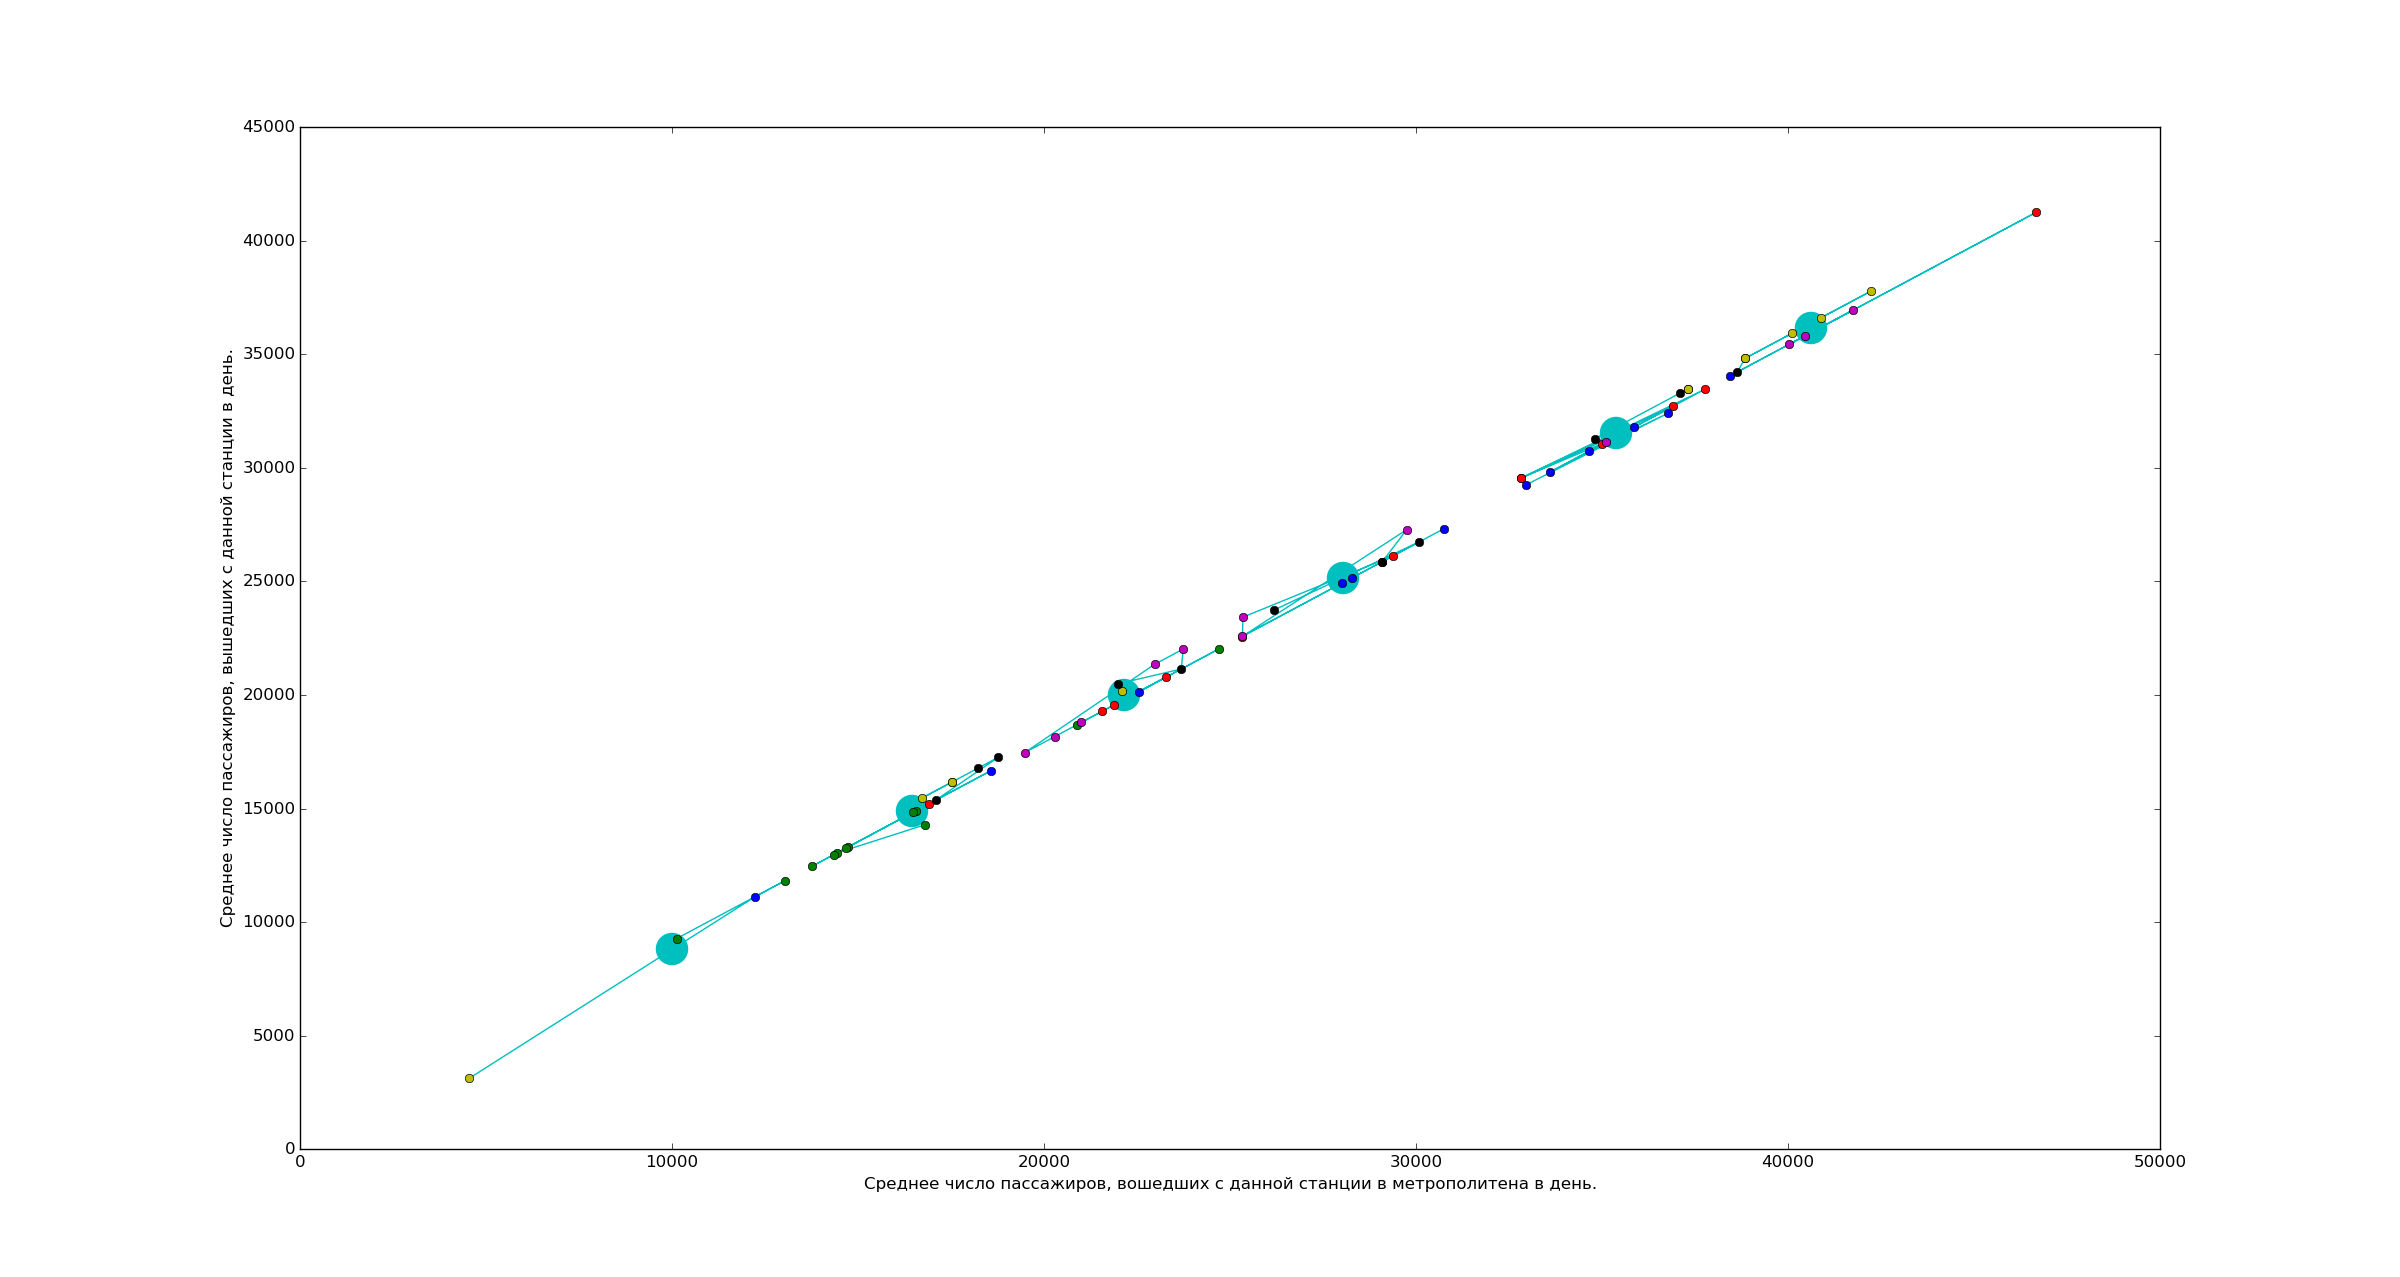
\includegraphics[scale=0.3]{figure_1.png}
            \caption{Визуализация результатов кластеризации}
            \label{pic:case1}
        \end{figure}

    \subsection{Cлучай 2}
        Были получены следующие результаты кластеризации --- каждому кластеру соответствует список станций метро в него попавших, которые разделены пробелами:
        \begin{enumerate}
            \item A0 A0 A1 A1 B0 B0 B0 B1 B1 B1 B1 B1 C0 C0 C0 C0 C1 
            \item A1 A1 B0 B0 B1 B1 C0 C0 C1 C1 C1 C1 C1 C1 
            \item A0 A0 A0 A0 A0 A0 A0 A0 A0 A0 A1 B0 C0 C1 C1 C1 C1 
            \item A1 A1 A1 A1 B0 B0 B0 B1 C0 
            \item B0 B1 C1 
            \item A1 A1 A1 B0 B0 B1 B1 B1 C0 C0 C0 C0
        \end{enumerate}

        Результаты провизуализированы на рисунке~\ref{pic:case2}. На нём большие голубые точки задают центры полученных кластеров, а голубые лини связывают между собой принадлежащие одному кластеру точки. Точки принадлежащие разным станциям метро, раскрашены разным цветом.

        \begin{figure}[ht!]
            \center
            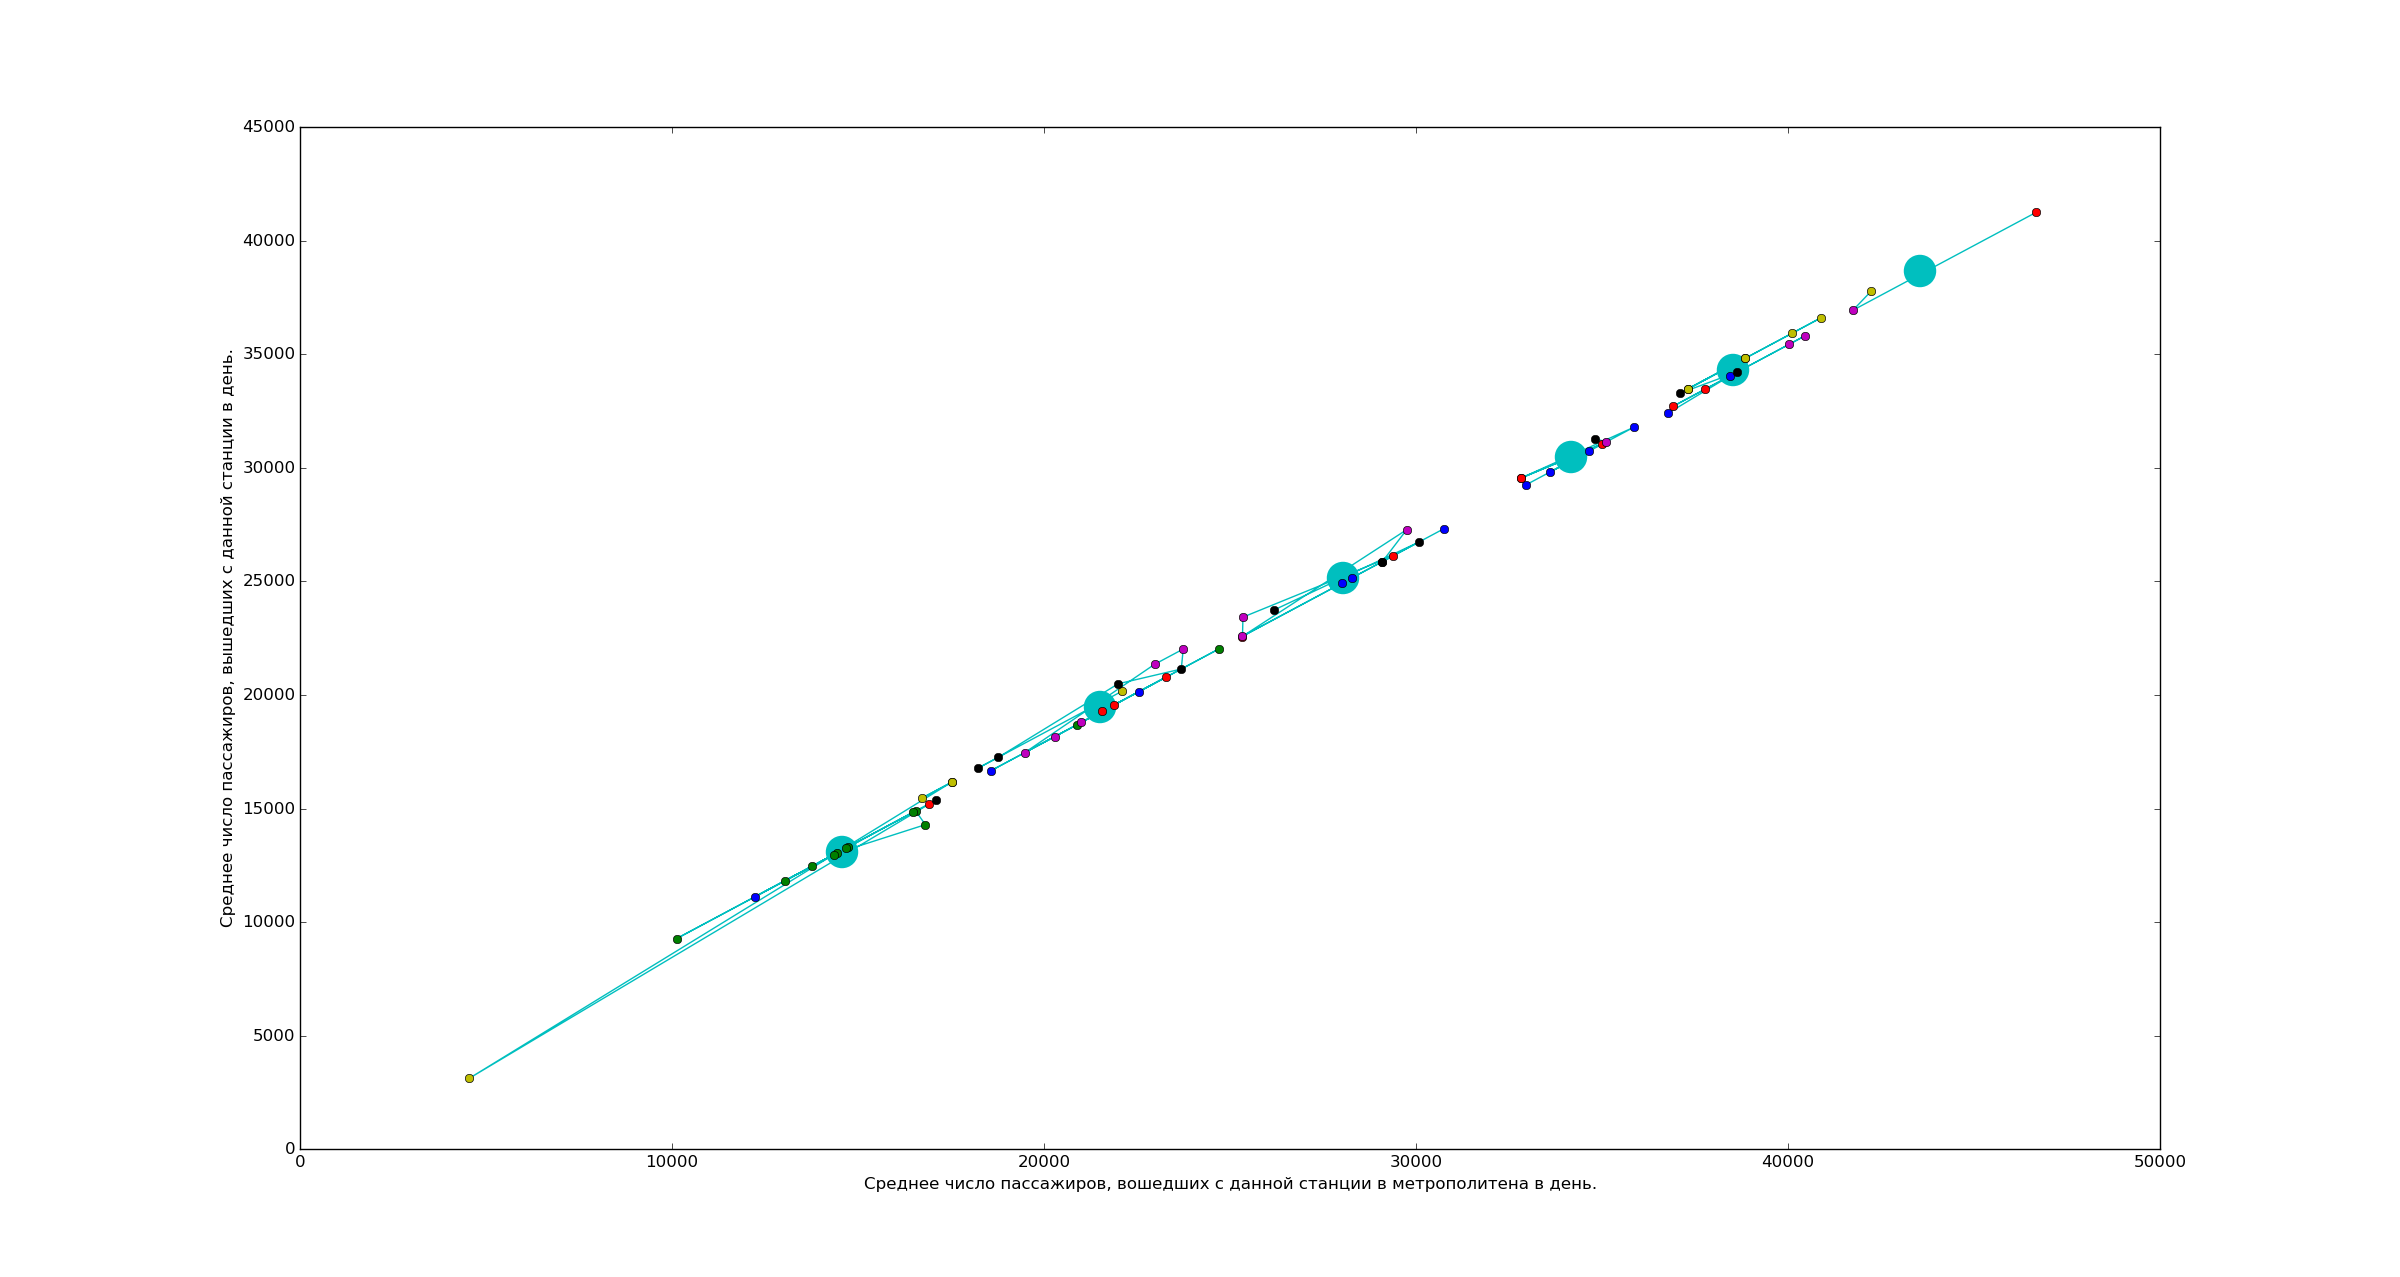
\includegraphics[scale=0.3]{figure_2.png}
            \caption{Визуализация результатов кластеризации}
            \label{pic:case2}
        \end{figure}

    Из результатов кластеризации видно, что в обоих случаях в целом кластеры не совпали с данными о станциях, что позволяет сделать вывод о сильной однородности входных данных. Также можно заметить, что достаточно много точек станции A0 (в первой случае 8, во втором 10) попали в рамки одного кластера, что говорит, об заметном отличии данных о стании A0, от остальных.
\end{document}
